\section{9. 3-SUM and Computational Geometry Problems}

\begin{df}[Convolution 3-SUM]
  Given three arrays $S_1, S_2, S_3$ (containing pairwise different integers) of size$n$.

  Check whether there are indices $1 \leq i, j, k \leq n$ such that

  \begin{equation*}
	\begin{cases}
	  S_1[i] + S_2[j] = S_3[k]\\
	  i + j = k
	\end{cases}
  \end{equation*}

  It is straightforward to solve Convolution 3-SUM in $O(n^2)$ just enumerate all $1 \leq i, j \leq n$.
\end{df}

\begin{thm}[Patrason, 2010; Chen-He, 2020]
  3-SUM $\to$ Convolution 3-SUM: if 3-SUM $\in T(n) \Longrightarrow$ Convolution 3-SUM $\in O(T(n) poly \log(n))$
\end{thm}
\begin{proof}
  Given $S_1, S_2, S_3$ instances for 3-SUM.

  For $S_1$ let's create $S_1'$ such that $\forall s \in S_1 : S_1'[s] = s$
  and simmilar for $S_2 \to S_2', \, S_3 \to S_3'$.

  Because integers of absolute value in $S_1, S_2, S_3$ not more than $n^3 \Longrightarrow |S_1'|, |S_2'|, |S_3'| \leq n^3$.

  In gaps we put some large numbers, just to be sure that they are not contribute to any sum.

  \begin{figure}[ht]
	\center
	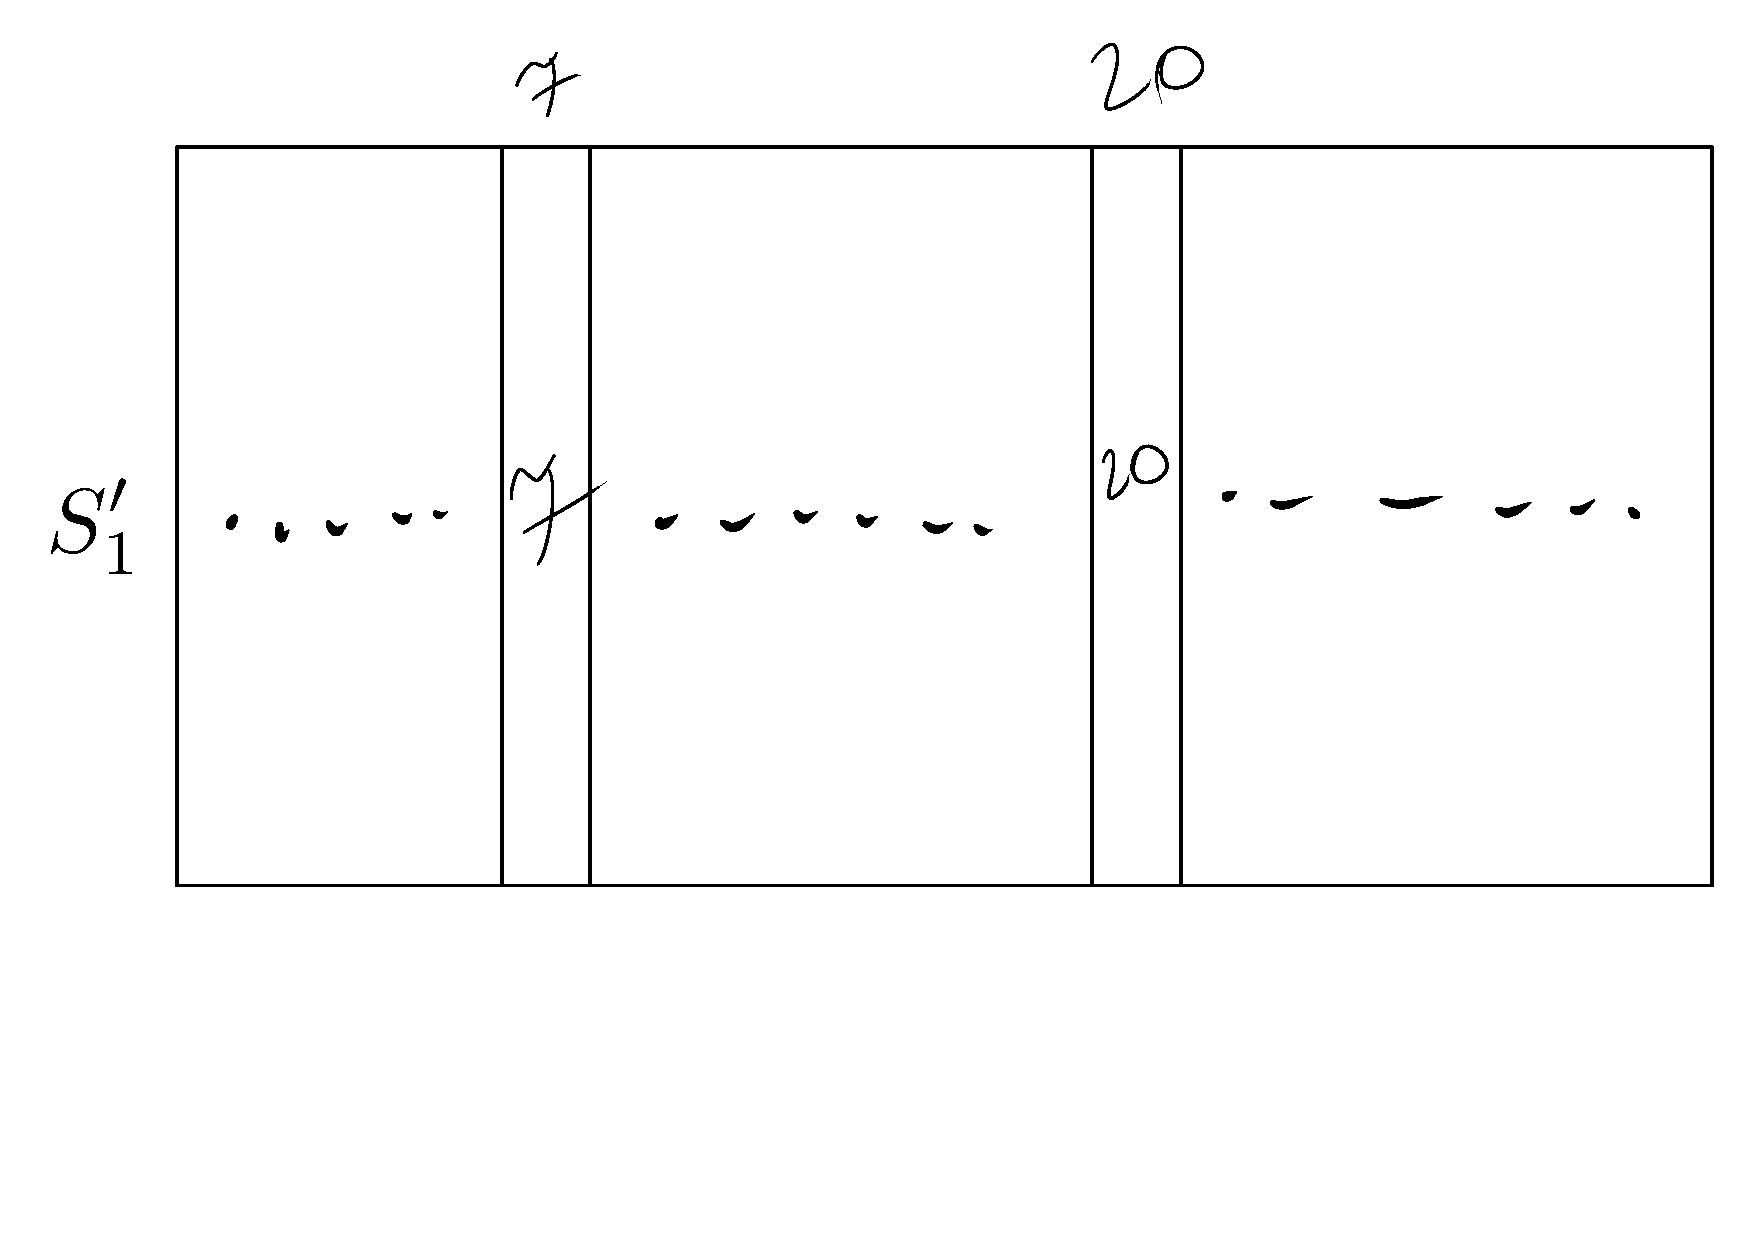
\includegraphics[scale=0.3]{figures/1.pdf}
	\caption{Example of $S_1'$ array}
  \end{figure}

  Our idea is to use some hash function $h$ of $s$ instead of just $s$.

  $S_1 \to S_1' : \forall s \in S_1 : S_1'[h(s)] = s$

  Desired properties of $h$:
  \begin{enumerate}
	\item linear: $h(s_1) + h(s_2) = h(s_1 + s_2)$
	\item range to be small: $h: [-n^3, n^3] \to R, |R| \leq \Ot(n)$
	\item number of collisions($s \neq s' : h(s) = h(s')$ ) to be small
  \end{enumerate}

  Constructing a hash function:

  take a random prime $p \leq 10 \cdot n \cdot \log^2 n$ and put $h(s) = s \mod p$.

  To get a random prime we use same idea as before cause number of a prime number is small enough.

  \begin{enumerate}
	\item almost linearity: for any $s_1, s_2 \Rightarrow h(s_1) + h(s_2) \in \{ h(s_1 + s_2), h(s_1 + s_2) + p \}$
	\item obviously
	\item we'll show how to deal with collisions.
	  for a remainder $r \mod p$ and a set $S$,
	  \begin{align*}
		S_r = \{s \in S: h(s) = s \mod p = r \}
	  \end{align*}


	  \begin{lstlisting}
Reduction algorithm($S_1, S_2, S_3$):
  Repeat $O(log(n))$  times:
	- generate a random prime $p <= 10 n \log n$
	- create arrays $S_1', S_2', S_3', S_3''$  with indeces $[0 \dots p)$:
		-for all $0 \leq r < p$:
			$S_1'[r]$  = random element of $(S_1)_r$
			same for $S_2', S_3'$
			$S_3''[r + p]$  = random element of $(S_3)_r$
	- if Convolution 3-SUM($S_1', S_2', S_3'$) = "yes" or
		Convolution 3-SUM($S_1', S_2', S_3''$) = "yes"
		return yes
return "no"
	  \end{lstlisting}

  \end{enumerate}

  \begin{figure}[ht]
	\center
	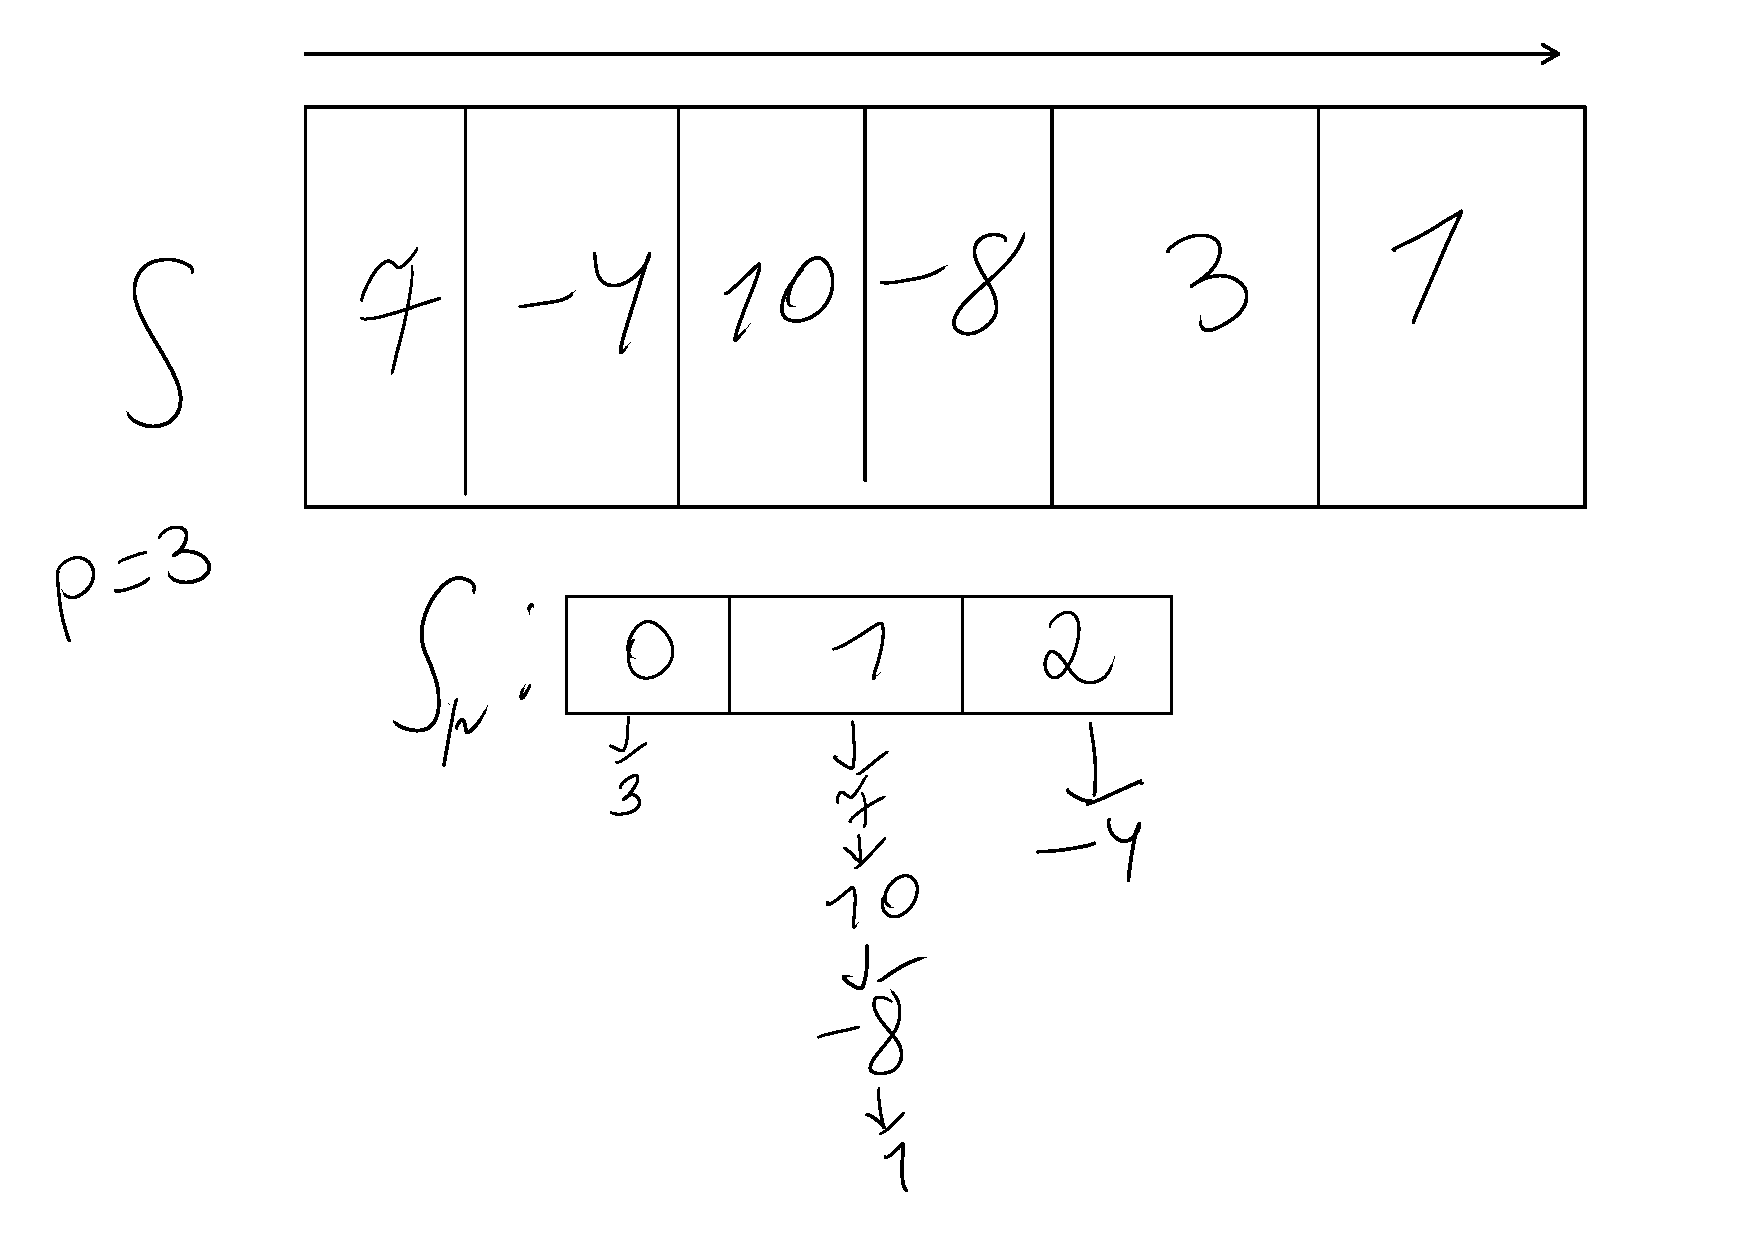
\includegraphics[scale=0.3]{figures/2.pdf}
	\caption{Example of $S_r$ array}
  \end{figure}

  \begin{thm}
	$Pr[\text{correct answer}] \geq 1 - \frac{1}{n}$ in point 3.
  \end{thm}
  \begin{proof}

	Cases:
	\begin{enumerate}
	  \item the algorithm returns "yes"
		\begin{align*}
		  Pr[\text{wrong answer}] = Pr[(S_1, S_2, S_3) \text{-no instance} \land ((S_1', S_2', S_3') \lor (S_1', S_2', S_3'') \text{yes}) ]
		\end{align*}
		\begin{figure}[ht]
		  \center
		  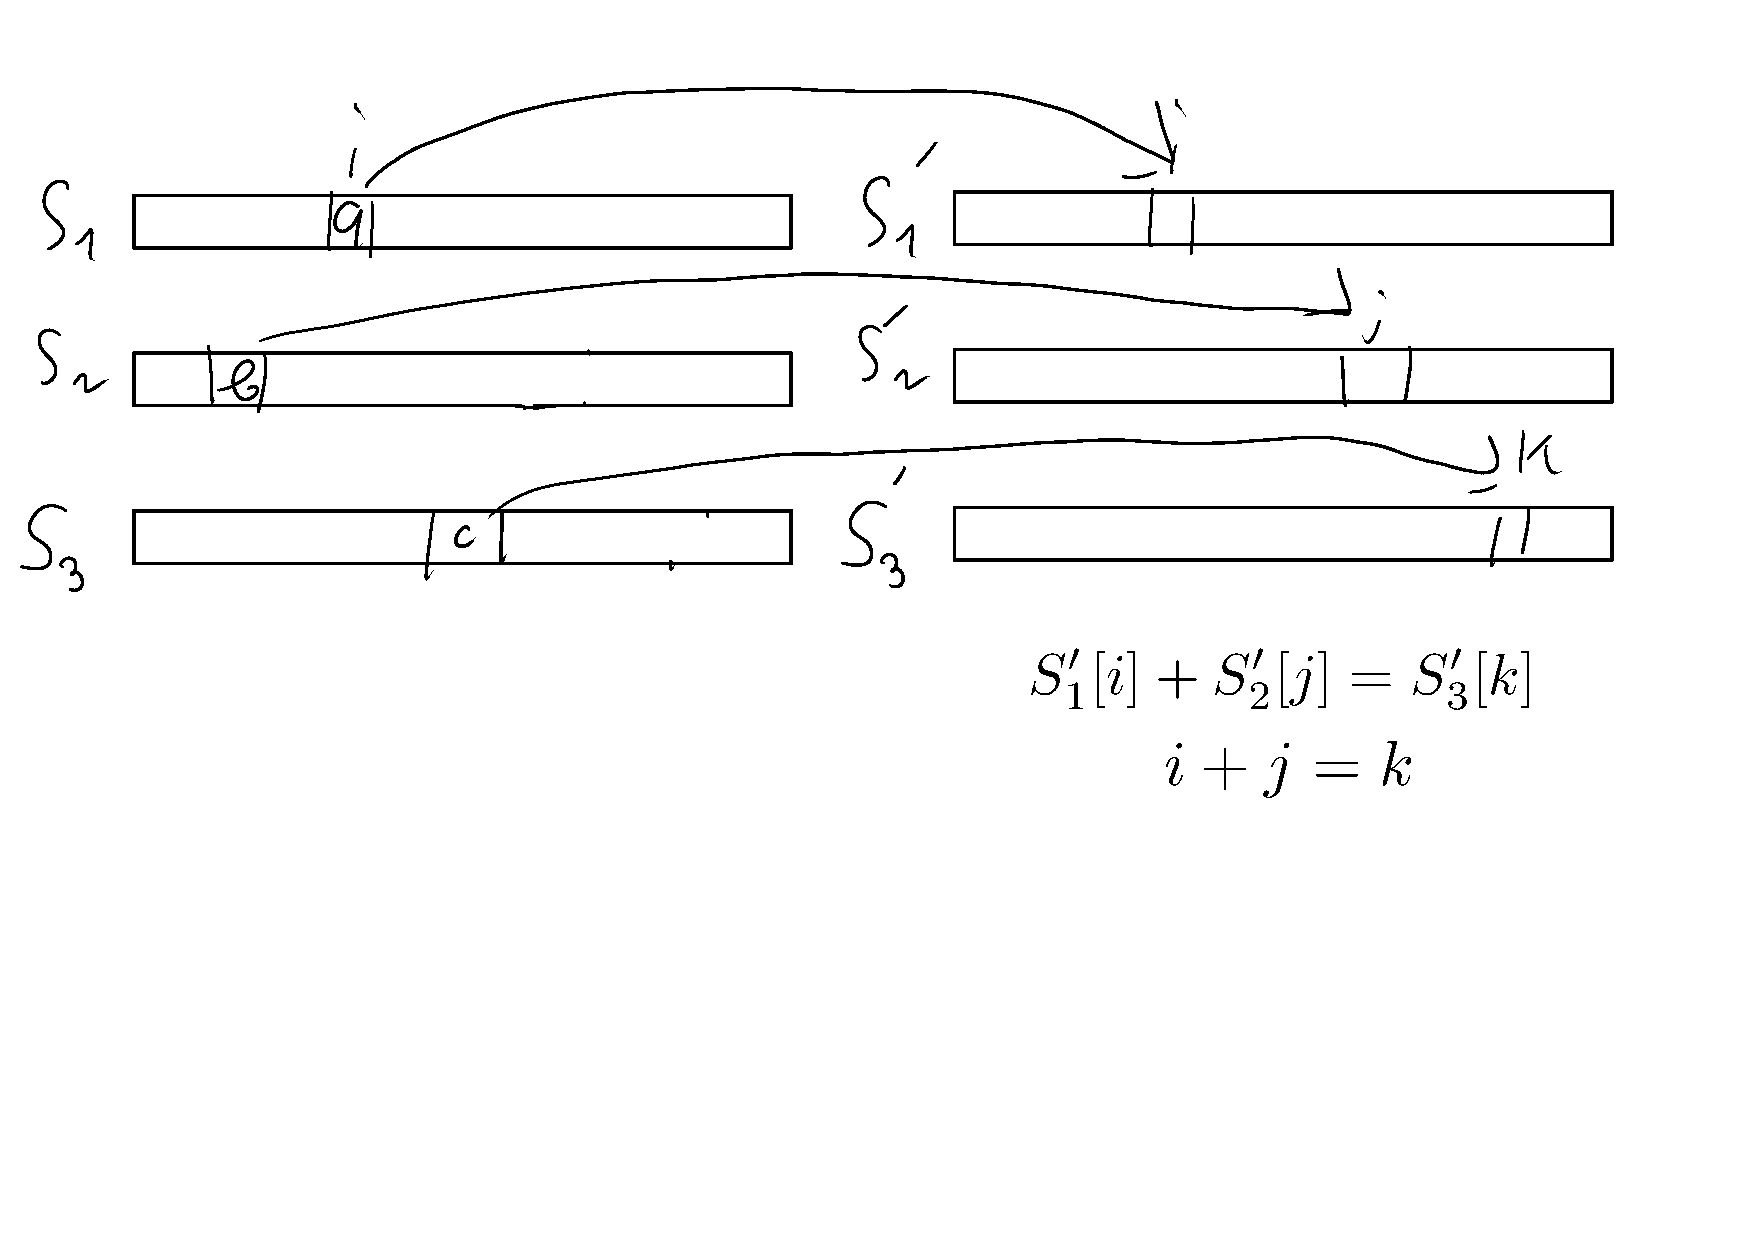
\includegraphics[scale=0.3]{figures/3.pdf}
		  \caption{First case pic.}
		\end{figure}


		Asume that $a, b, c$ is fixed tuple and $a + b \neq c$.

		\begin{align*}
		  Pr[(a + b) \mod p = c \mod p] = Pr[(a + b - c) \mod p = 0] \leq \\
		  \leq \frac{3 \cdot \log n}{10 \cdot n \cdot \log^2 n / \ln(10 \cdot n \cdot \log^2 n)} \leq \frac{1}{n}
		\end{align*}

		{\color{red} We will end proof on the next lecture}

	  \item the algorithm return "no".

		This answer is incorrect if $\exists s_1 \in S_1, s_2 \in S_2, s_3 \in S_3 : s_1 + s_2 = s_3$, but this triple $(s_1, s_2, s_3)$ does not survive during sampling random elements.

		We are going to show that the triple $(s_1, s_2, s_3)$ is sampled with good enough probability.

		Notation: $s \in S$ is $S$-good if $|S_r| \leq 10$ where $r = s \mod p$ and $S$-bad otherwise.

		$s \in S$ is $S$-chosn if $s$ is selected when sampling a random representative.

		We are going to show that 

		\begin{align*}
		  Pr[s_1 \text{ is }S_1\text{-chosen}, s_2 \text{ is }S_2\text{-chosen}, s_3 \text{is } s_3\text{ is } S_3\text{-chosen}]
		\end{align*}
		is large enough.

		\begin{align*}
		  Pr[s \text{ is }S\text{-bad}] \leq ?
		\end{align*}

		Fix $s' \in S$ such that $s \neq s'$:

		\begin{align*}
		  Pr[s \ mod \ p = s' \ mod \ p] \leq \frac{\text{\# prime divisors}}{\text{\# primes}} \leq \frac{3\log n}{10 \cdot n \cdot \log^2 n / \ln(10 \cdot n \log^2 n)} \leq \frac{1}{3 n}
		\end{align*}

		That means for $s \in S$ the expected number of elements of $S$ that have the same hash value is $\frac{1}{3} \Longrightarrow Pr[s \text{ is } S\text{-bad}] \leq \frac{1}{30}$ by Markov's inequality.


		\begin{align*}
		  Pr[s \text{ is } S\text{-chosen } | s \text{ is  } S\text{-good}] \geq \frac{1}{10} \\
		  Pr[s \text { is } S\text{-chosen}] \geq Pr[s \text{ is } S\text{-chosen} | s \text{ is } S\text{-good}] \cdot Pr[s \text { is } S\text{-good}] \geq \\
		  \geq \frac{1}{10} \cdot \frac{29}{30} = \frac{29}{300} \geq \frac{1}{15} \\
		  Pr[s_1 \text{ is }S_1\text{-chosen}, s_2 \text{ is }S_2\text{-chosen}, s_3 \text{is } s_3\text{ is } S_3\text{-chosen}] \geq \left(\frac{1}{15}\right)^{3}
		\end{align*}

	\end{enumerate}
  \end{proof}



\end{proof}

